\documentclass[12pt,a4paper]{article}

% --- Codificacion, idioma y tipografia (Times New Roman igual que 2o parcial.pdf) ---
\usepackage[utf8]{inputenc}
\usepackage[T1]{fontenc}
\usepackage[spanish,es-nodecimaldot,es-tabla]{babel}
\usepackage{newtxtext,newtxmath}

% --- Geometria A4 y margenes equivalentes al PDF del examen ---
\usepackage[a4paper, left=3cm, right=2.9cm, top=2.1cm, bottom=2.4cm]{geometry}

% --- Paquetes auxiliares para figuras, tablas, formulas y formato ---
\usepackage{graphicx}
\usepackage{float}
\usepackage{booktabs}
\usepackage{array}
\usepackage{amsmath}
\usepackage{enumitem}
\usepackage{fancyhdr}
\usepackage{caption}
\usepackage[hidelinks]{hyperref}

% --- Configuracion de figuras y tablas ---
\captionsetup{
    font=small,
    labelfont=bf,
    justification=centering
}

% --- Encabezado y pie de pagina discretos en el cuerpo del documento ---
\pagestyle{fancy}
\fancyhf{}
\fancyhead[L]{\small BUAP -- FCC}
\fancyhead[R]{\small Minería de Datos -- 2o parcial}
\fancyfoot[C]{\small\thepage}
\renewcommand{\headrulewidth}{0.4pt}

\begin{document}

% ==============================================================================
% PORTADA
% ==============================================================================
\begin{titlepage}
    \thispagestyle{empty}
    \begin{center}
        % Fila superior con los escudos de la Universidad y de la Facultad
        \noindent
        \begin{minipage}[c]{0.22\textwidth}
            \centering
            \IfFileExists{Escudos/escudo_buap.png}{%
                
\includegraphics[height=2.5cm, keepaspectratio]{Escudos/escudo_buap.png}%
            }{%
                \IfFileExists{Escudos/escudo_buap.jpg}{%
                    \includegraphics[height=2.5cm, keepaspectratio]{Escudos/escudo_buap.jpg}%
                }{%
                    \fbox{\parbox[c][2.3cm][c]{2.2cm}{\centering\small Escudo\\BUAP}}%
                }%
            }
        \end{minipage}
        \hfill
        \begin{minipage}[c]{0.52\textwidth}
            \centering
            {\Large \textbf{BENEMÉRITA UNIVERSIDAD AUTÓNOMA DE PUEBLA}}\\[0.3cm]
            {\large \textbf{FACULTAD DE CIENCIAS DE LA COMPUTACIÓN}}
        \end{minipage}
        \hfill
        \begin{minipage}[c]{0.22\textwidth}
            \centering
            \IfFileExists{Escudos/escudo_fcc.png}{%
                
\includegraphics[height=2.5cm, keepaspectratio]{Escudos/escudo_fcc.png}%
            }{%
                \IfFileExists{Escudos/escudo_fcc.jpg}{%
                    \includegraphics[height=2.5cm, keepaspectratio]{Escudos/escudo_fcc.jpg}%
                }{%
                    \fbox{\parbox[c][2.3cm][c]{2.2cm}{\centering\small Escudo\\FCC}}%
                }%
            }
        \end{minipage}

        \vspace{2.2cm}

        \rule{\textwidth}{0.8pt}\\[0.5cm]
        {\LARGE \textbf{2o parcial}}\\[0.25cm]
        {\large \textbf{Minería de Datos}}\\[0.35cm]
        \rule{\textwidth}{0.8pt}

        \vspace{1.2cm}

        {\large
        Modelo de Clasificación Basado en Redes Neuronales Artificiales (RNA)\\
        sobre Clusters Identificados con el Algoritmo DBSCAN
        }

        \vspace{2.2cm}

        \textbf{Integrantes (ordenados por apellido paterno):}\\[0.5cm]
        \begin{tabular}{@{} p{8.8cm} c @{}}
            \toprule
            \textbf{Nombre del alumno} & \textbf{Matrícula} \\
            \midrule
            1. Arias Santos Angelica Alejandra & 202236284 \\[0.25cm]
            2. Ramiro Luna Luis Emmanuel & 202352409 \\[0.25cm]
            3. Soto Gonzalez Edgar & 202357286 \\
            \bottomrule
        \end{tabular}

        \vfill

        \textbf{Fecha de entrega:} 29 de noviembre
    \end{center}
\end{titlepage}

% ==============================================================================
% ENCABEZADO DEL EXAMEN (ESTILO IDENTICO AL PDF ORIGINAL)
% ==============================================================================
\begin{center}
    BUAP - FCC \\
    \textbf{2o parcial}
\end{center}

\vspace{0.4cm}

{\footnotesize
\noindent \textbf{Instrucciones}: Analiza cada una de las preguntas que se exponen a continuación. Realiza las implementaciones correspondientes, las cuales se deberán de entregar en la fecha indicada. En caso de duda, favor de contactar al profesor.
}

\vspace{0.35cm}

\noindent Construye un modelo de clasificación basado en una RNA que modele el comportamiento de los clusters identificado con el algoritmo DBSCAN a partir de la base de datos propuesta. Para ello, considera las siguientes etapas:

\vspace{0.4cm}

% ==============================================================================
% PREGUNTA 1 (ENUNCIADO EXACTO DEL EXAMEN)
% ==============================================================================
\begin{enumerate}[leftmargin=1.1cm, label=\textbf{\arabic*.}]
    \item \textbf{(2.5)} Realizar e implementar una etapa de preprocesamiento a la base de datos propuesta, de tal forma que se eliminen diferentes tipos de problemas del dataset, como ruido, desviaciones, etc. Se deberá de usar un algoritmo de agrupamiento (DBSCAN), para la detección de ruido tipo global, ajustándolo de acuerdo a los requerimientos del dataset (se deberá de elegir las métricas para medir la calidad de los estratos generados). Se debe documentar cómo se ha aplicado el algoritmo al problema. Se deberá generar un archivo denominado ``preprocesamiento.py''. A los grupos generados por esta etapa, asignarles un valor de clase.
\end{enumerate}

% ==============================================================================
% RESPUESTA Y DESARROLLO DEL INCISO 1
% ==============================================================================
\subsection*{Desarrollo y Respuesta -- Etapa 1: Preprocesamiento}

Para dar cumplimiento a la Etapa 1 del examen, el trabajo se dividió en dos fases complementarias: primero, un análisis exploratorio exhaustivo del archivo original \texttt{Dataset.csv} para diagnosticar sus problemas de calidad y definir el plan de limpieza; y segundo, la implementación automatizada en el script \texttt{preprocesamiento.py}.

\subsubsection*{1. Diagnóstico Inicial del Dataset (\texttt{Dataset.csv})}

El conjunto de datos original está compuesto por \textbf{13,611 registros} de granos y \textbf{17 columnas}, de las cuales 16 corresponden a atributos morfológicos y geométricos numéricos (\texttt{Area}, \texttt{Perimeter}, \texttt{MajorAxisLength}, \texttt{MinorAxisLength}, \texttt{AspectRation}, \texttt{Eccentricity}, \texttt{ConvexArea}, \texttt{EquivDiameter}, \texttt{Extent}, \texttt{Solidity}, \texttt{roundness}, \texttt{Compactness} y \texttt{ShapeFactor1} a \texttt{ShapeFactor4}).

Al inspeccionar la calidad e integridad de los datos antes de realizar transformaciones (Figura~\ref{fig:calidad_nulos}), se identificaron los siguientes hallazgos:

\begin{itemize}[leftmargin=0.8cm]
    \item \textbf{Columna vacía residual (\texttt{Unnamed: 16}):} El archivo contiene una columna extra al final generada por una coma terminal en las líneas del CSV, con \textbf{13,611 valores nulos (100\% vacía)}. Las 16 variables reales del grano no presentan valores faltantes (0 nulos).
    \item \textbf{Registros duplicados exactos:} Se detectaron \textbf{68 filas repetidas (0.50\%)} y 13,543 registros únicos (99.50\%). Eliminar estos duplicados es fundamental para evitar que inflen artificialmente la densidad local al aplicar DBSCAN.
    \item \textbf{Varianza de las variables:} Todas las 16 variables numéricas poseen varianza estrictamente mayor que cero (no existen columnas constantes).
\end{itemize}

\begin{figure}[H]
    \centering
    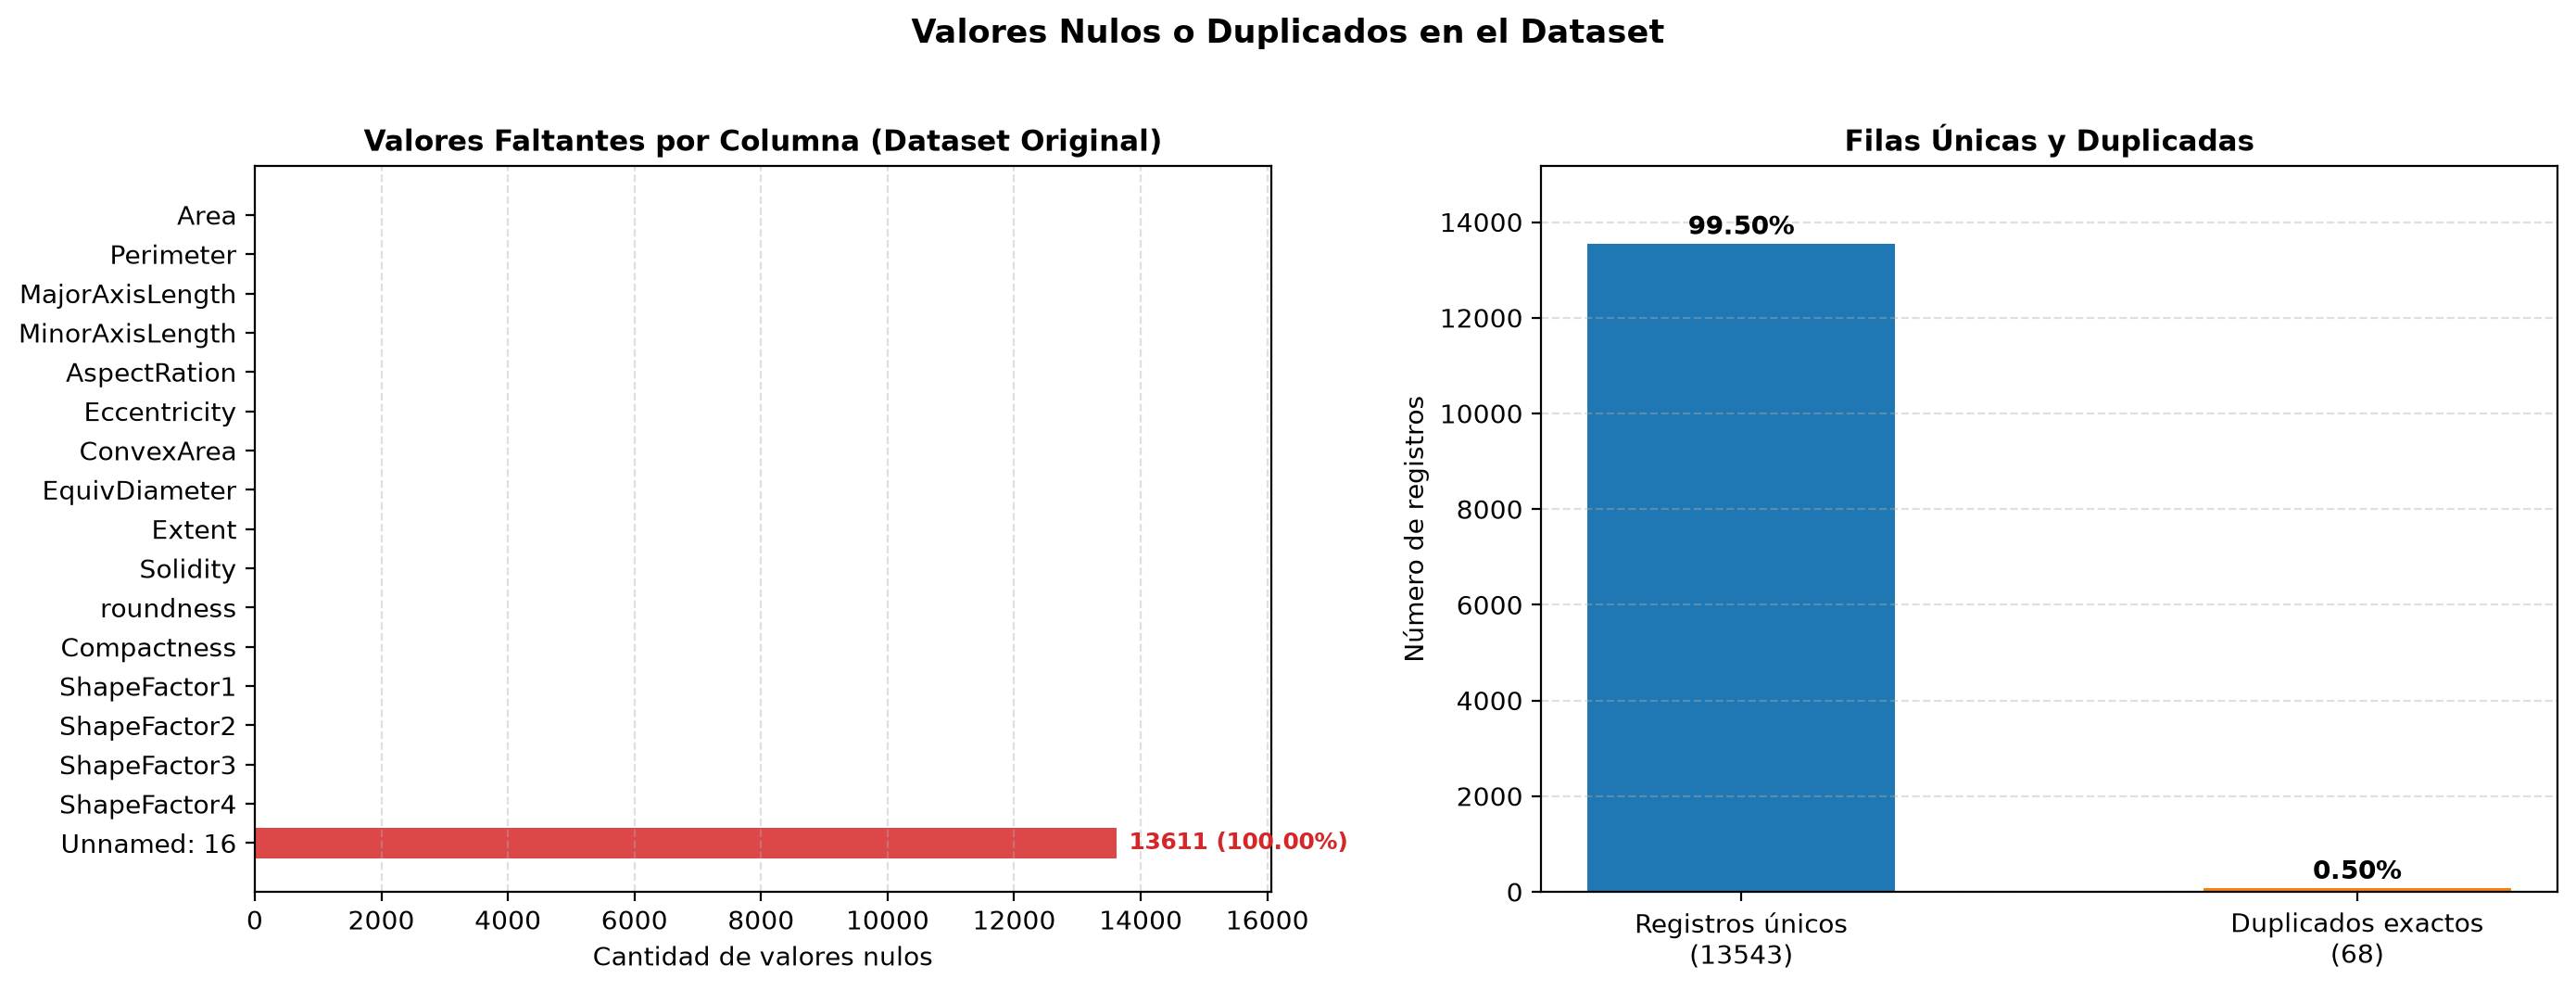
\includegraphics[width=0.95\textwidth]{Inciso_1/1_calidad_y_nulos.png}
    \caption{Diagnóstico de valores faltantes por columna y proporción de registros duplicados en el dataset original.}
    \label{fig:calidad_nulos}
\end{figure}

Posteriormente, se analizaron las distribuciones individuales de las 16 variables en su escala original (Figura~\ref{fig:histogramas}). Esta gráfica evidenció tres características clave:

\begin{enumerate}[leftmargin=0.8cm]
    \item \textbf{Disparidad extrema de escalas:} Variables de tamaño como \texttt{Area} oscilan entre $20{,}420.0$ y $254{,}616.0$ píxeles (y \texttt{ConvexArea} alcanza $263{,}261.0$), mientras que los factores de forma como \texttt{ShapeFactor2} toman valores entre $0.00056$ y $0.00366$. Sin estandarización previa, el cálculo de distancias euclidianas quedaría completamente dominado por \texttt{Area}.
    \item \textbf{Distribuciones multimodales:} Atributos como \texttt{MajorAxisLength}, \texttt{AspectRation}, \texttt{Compactness} y \texttt{ShapeFactor2} muestran múltiples picos, reflejando la presencia de distintos tipos de granos, además de un grupo bien diferenciado de granos grandes a la derecha (\texttt{Area} $> 125{,}000$).
    \item \textbf{Colas hacia valores extremos:} Variables de regularidad como \texttt{Solidity} ($0.9192$ a $0.9947$) y \texttt{ShapeFactor4} ($0.9477$ a $0.9997$) concentran la mayoría de los granos cerca de $0.99$, pero muestran una cola hacia valores bajos asociada a granos irregulares o posible ruido.
\end{enumerate}

\begin{figure}[H]
    \centering
    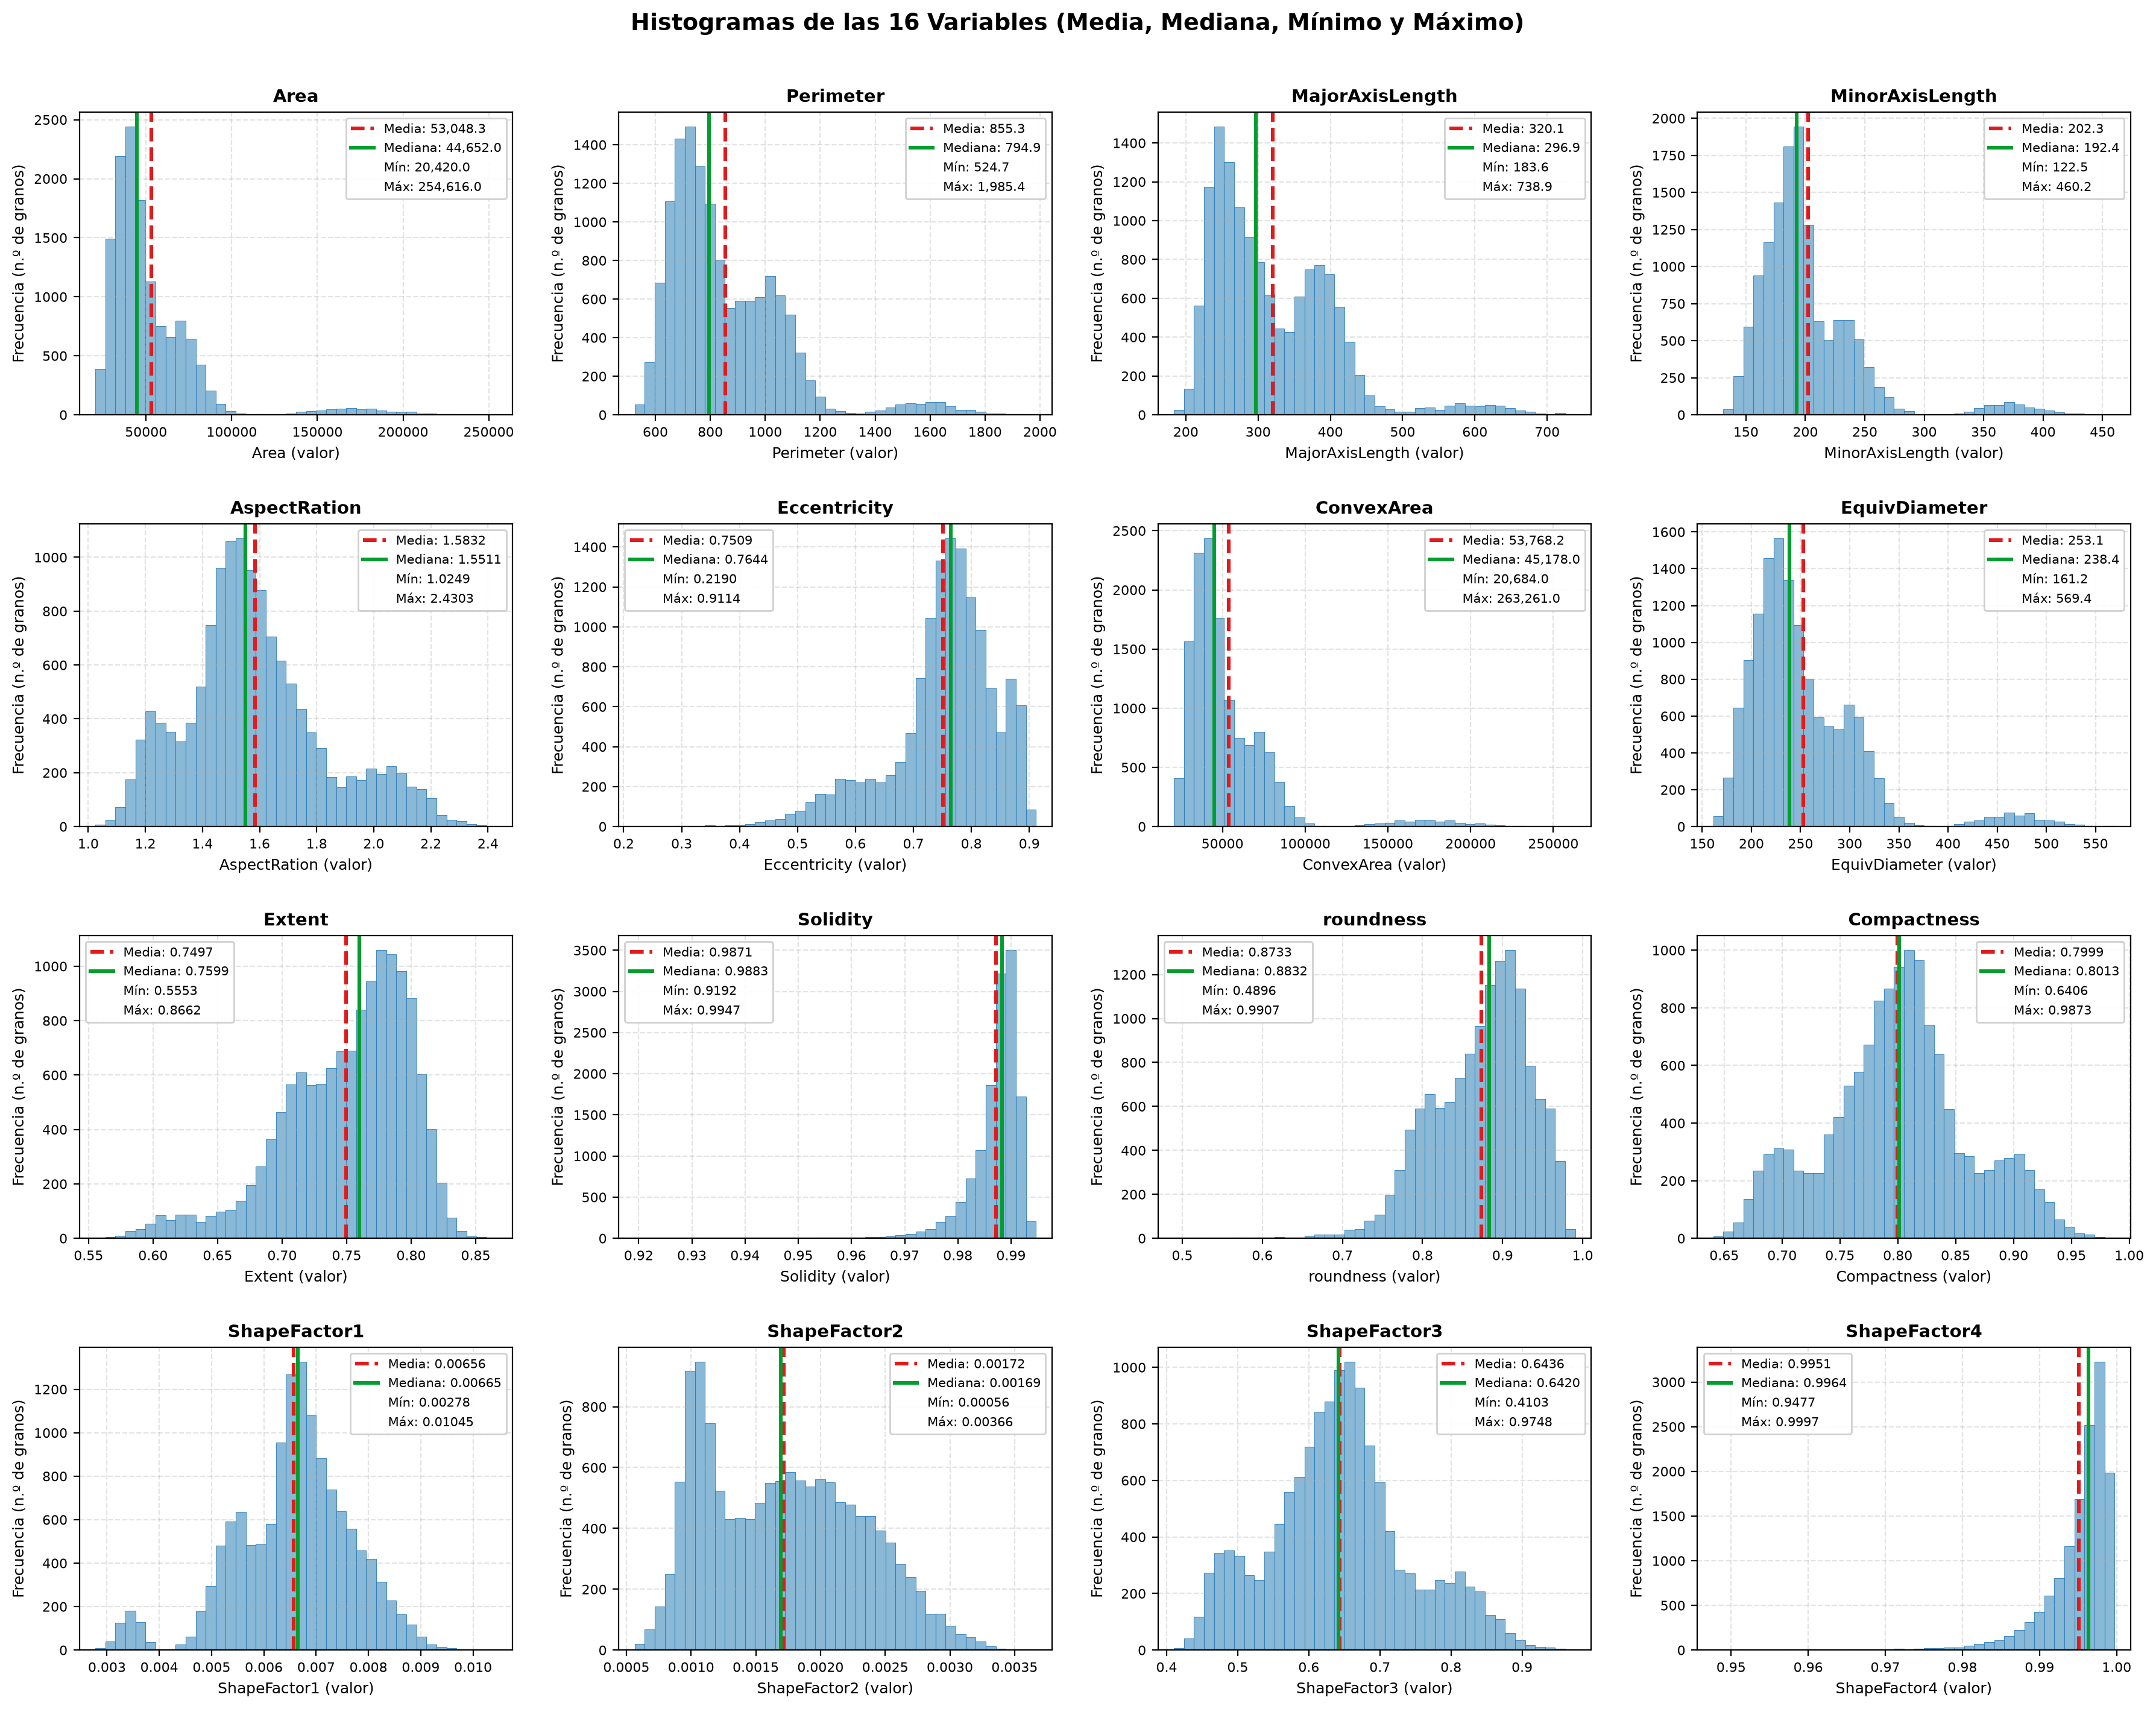
\includegraphics[width=0.98\textwidth]{Inciso_1/2_distribuciones_histogramas.png}
    \caption{Histogramas de las 16 variables en su escala original mostrando media, mediana, mínimo y máximo.}
    \label{fig:histogramas}
\end{figure}

También se calculó la matriz de correlación lineal de Pearson (Figura~\ref{fig:correlacion}), identificando bloques con correlación muy fuerte ($|r| > 0.95$) entre variables de tamaño (\texttt{Area} y \texttt{ConvexArea} con $r = 0.9999$; \texttt{Perimeter} y \texttt{EquivDiameter} con $r = 0.9914$) y de forma (\texttt{Compactness} y \texttt{ShapeFactor3} con $r = 0.9987$).

A pesar de esta redundancia lineal, se decidió \textbf{conservar las 16 variables originales} por tres razones:
\begin{enumerate}[leftmargin=0.8cm]
    \item En esta etapa no existe una etiqueta previa de \texttt{Clase} contra la cual evaluar qué variable predictora descartar sin sesgo.
    \item Las pequeñas diferencias entre atributos altamente correlacionados (como entre \texttt{Area} y \texttt{ConvexArea}) son útiles para detectar granos deformes o rotos en la identificación de ruido.
    \item El modelo final será una Red Neuronal Multicapa (MLP), arquitectura que gestiona adecuadamente atributos correlacionados mediante el ajuste de pesos y la regularización.
\end{enumerate}

\begin{figure}[H]
    \centering
    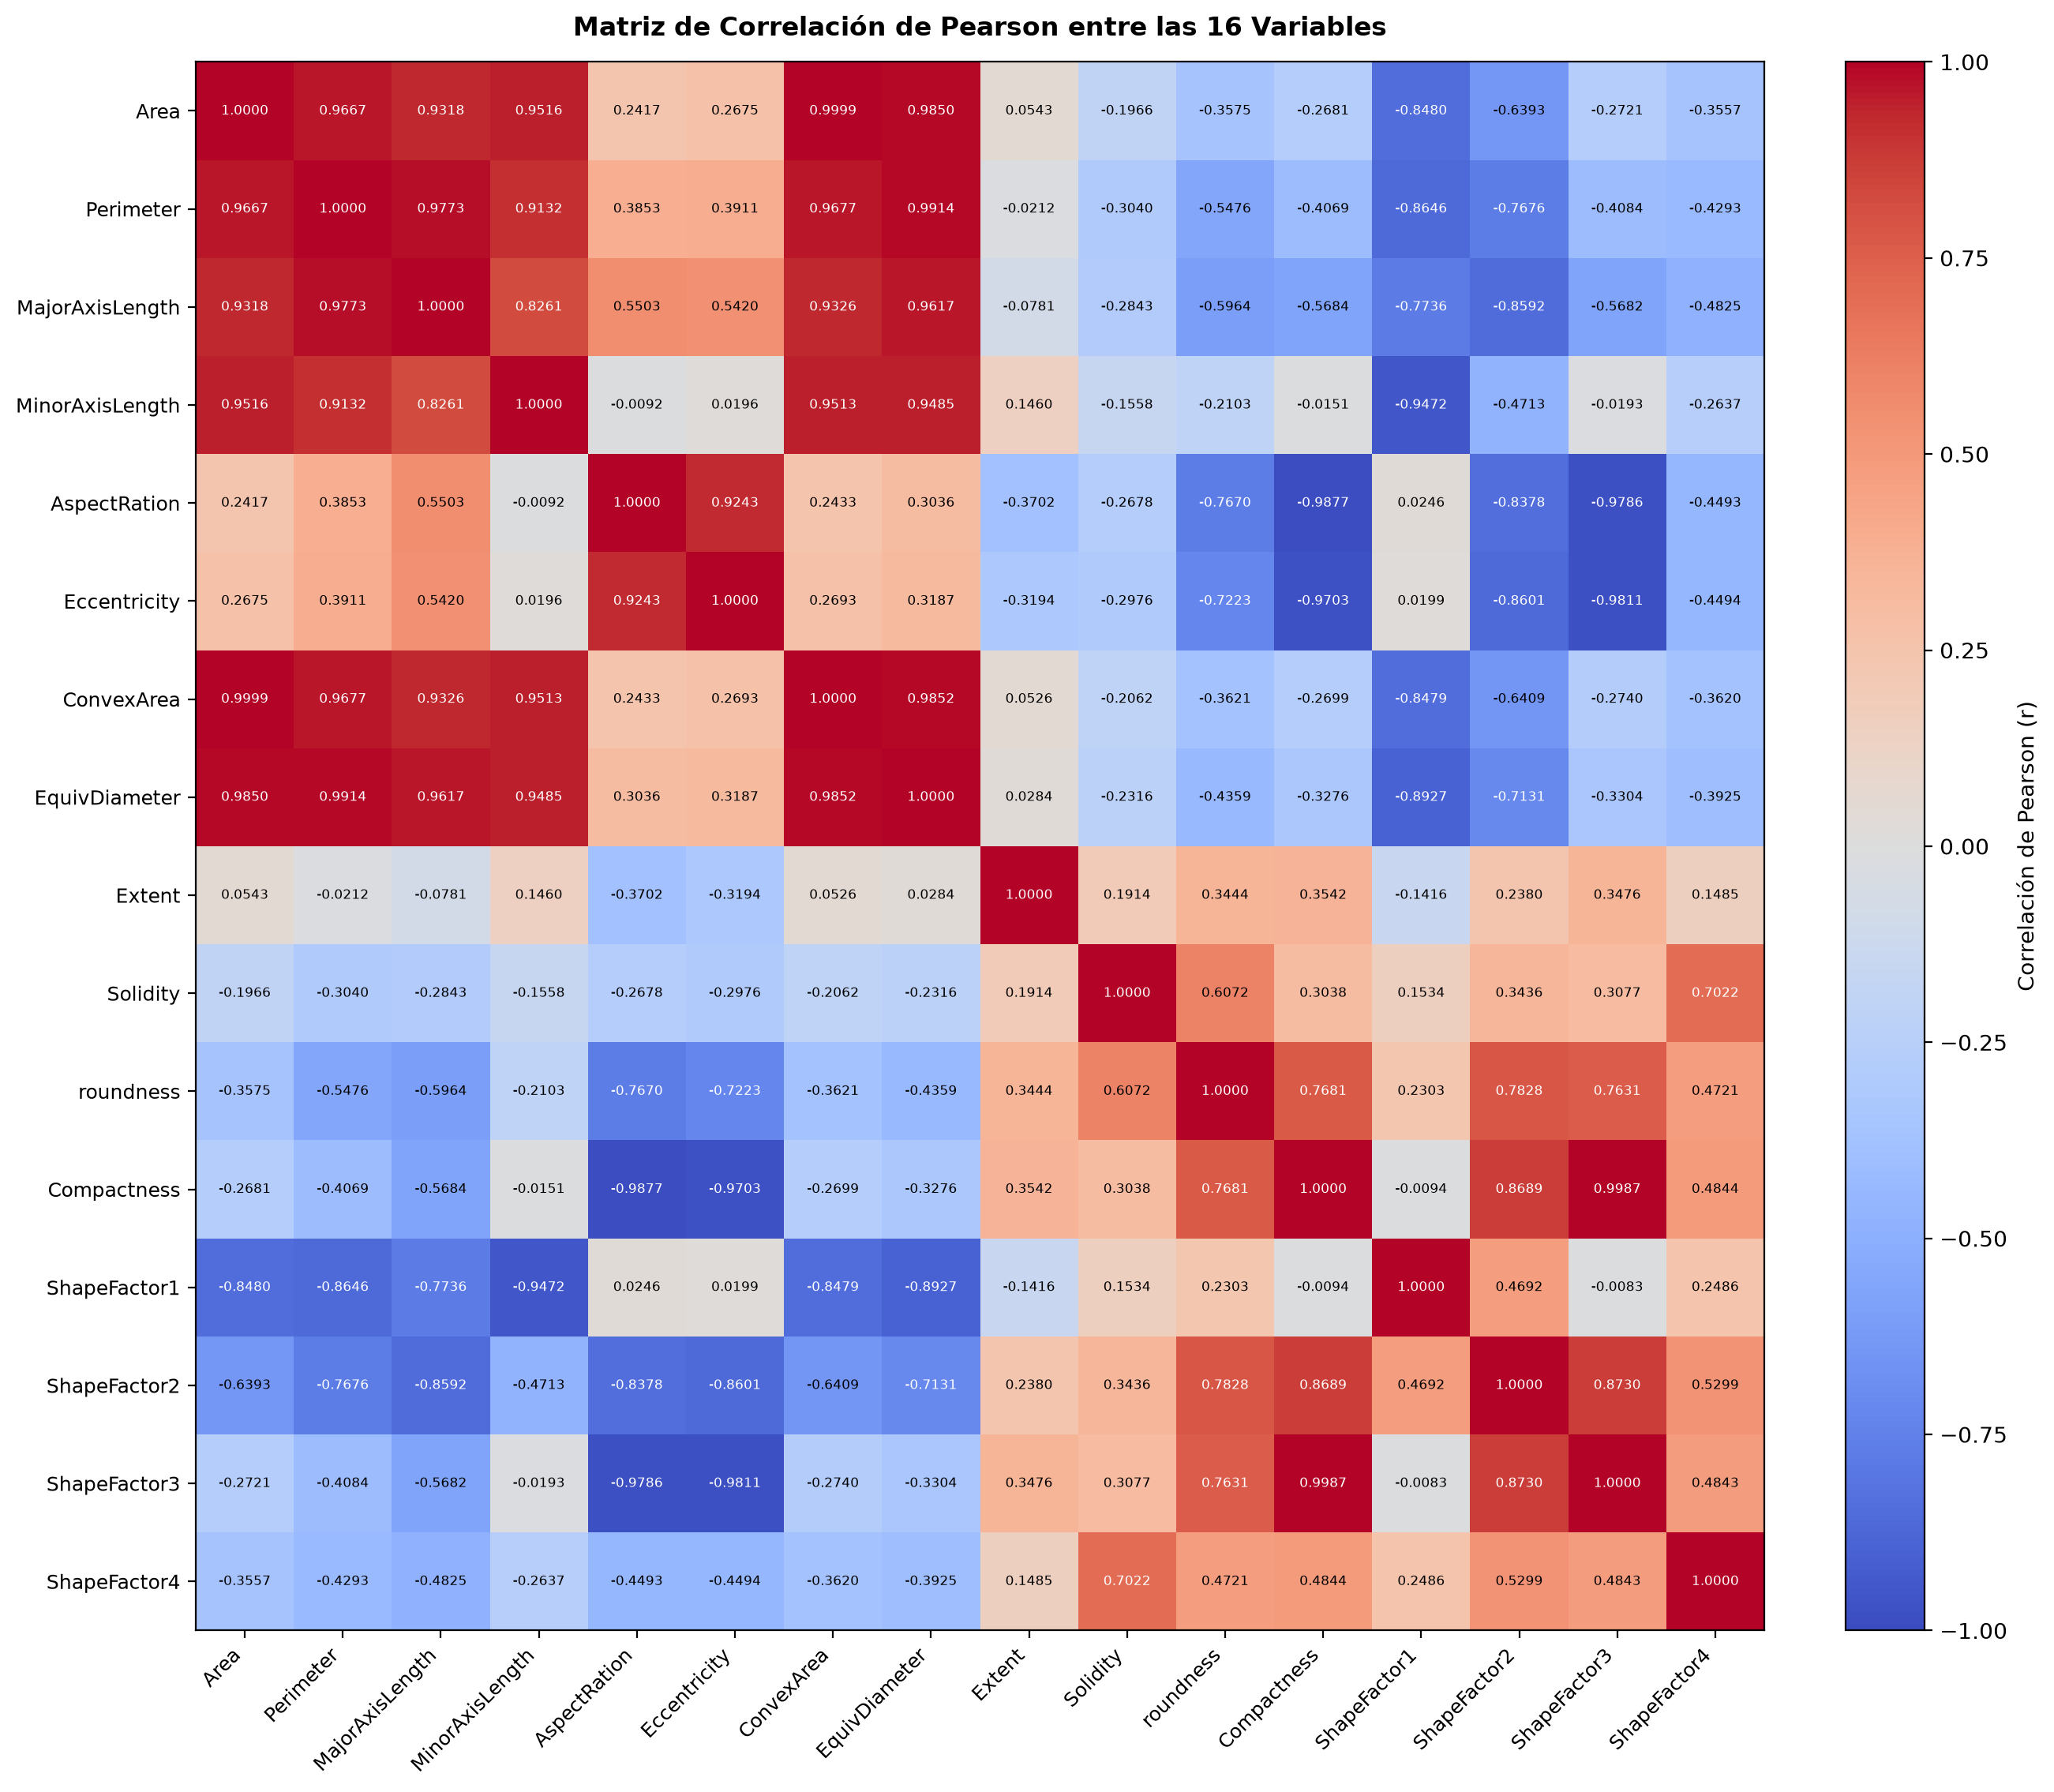
\includegraphics[width=0.88\textwidth]{Inciso_1/3_matriz_correlacion.png}
    \caption{Matriz de correlación lineal de Pearson entre las 16 variables numéricas del dataset.}
    \label{fig:correlacion}
\end{figure}

Finalmente, como no es posible visualizar directamente un espacio de 16 dimensiones, se generó una proyección exploratoria mediante Análisis de Componentes Principales (PCA) en 2D junto con un mapa de densidad hexagonal (Figura~\ref{fig:pca_analisis}). Los dos primeros componentes (\texttt{PC1} $= 55.47\%$ y \texttt{PC2} $= 26.43\%$) conservan el \textbf{81.90\% de la varianza total}. Esta proyección se empleó únicamente como herramienta visual (sin reducir las 16 dimensiones para el preprocesamiento) y permitió observar:
\begin{itemize}[leftmargin=0.8cm]
    \item Cuatro núcleos de muy alta densidad en la parte inferior izquierda que permanecen conectados entre sí por zonas grises intermedias.
    \item Una nube separada en la zona superior derecha que, aunque se visualiza en tonos grises más claros por tener menor cantidad de registros, agrupa a más de 400 granos de gran tamaño y no constituye ruido.
    \item Puntos aislados en los bordes exteriores (celdas pálidas con apenas 1 o 2 registros), correspondientes al \textbf{ruido global}.
\end{itemize}

\begin{figure}[H]
    \centering
    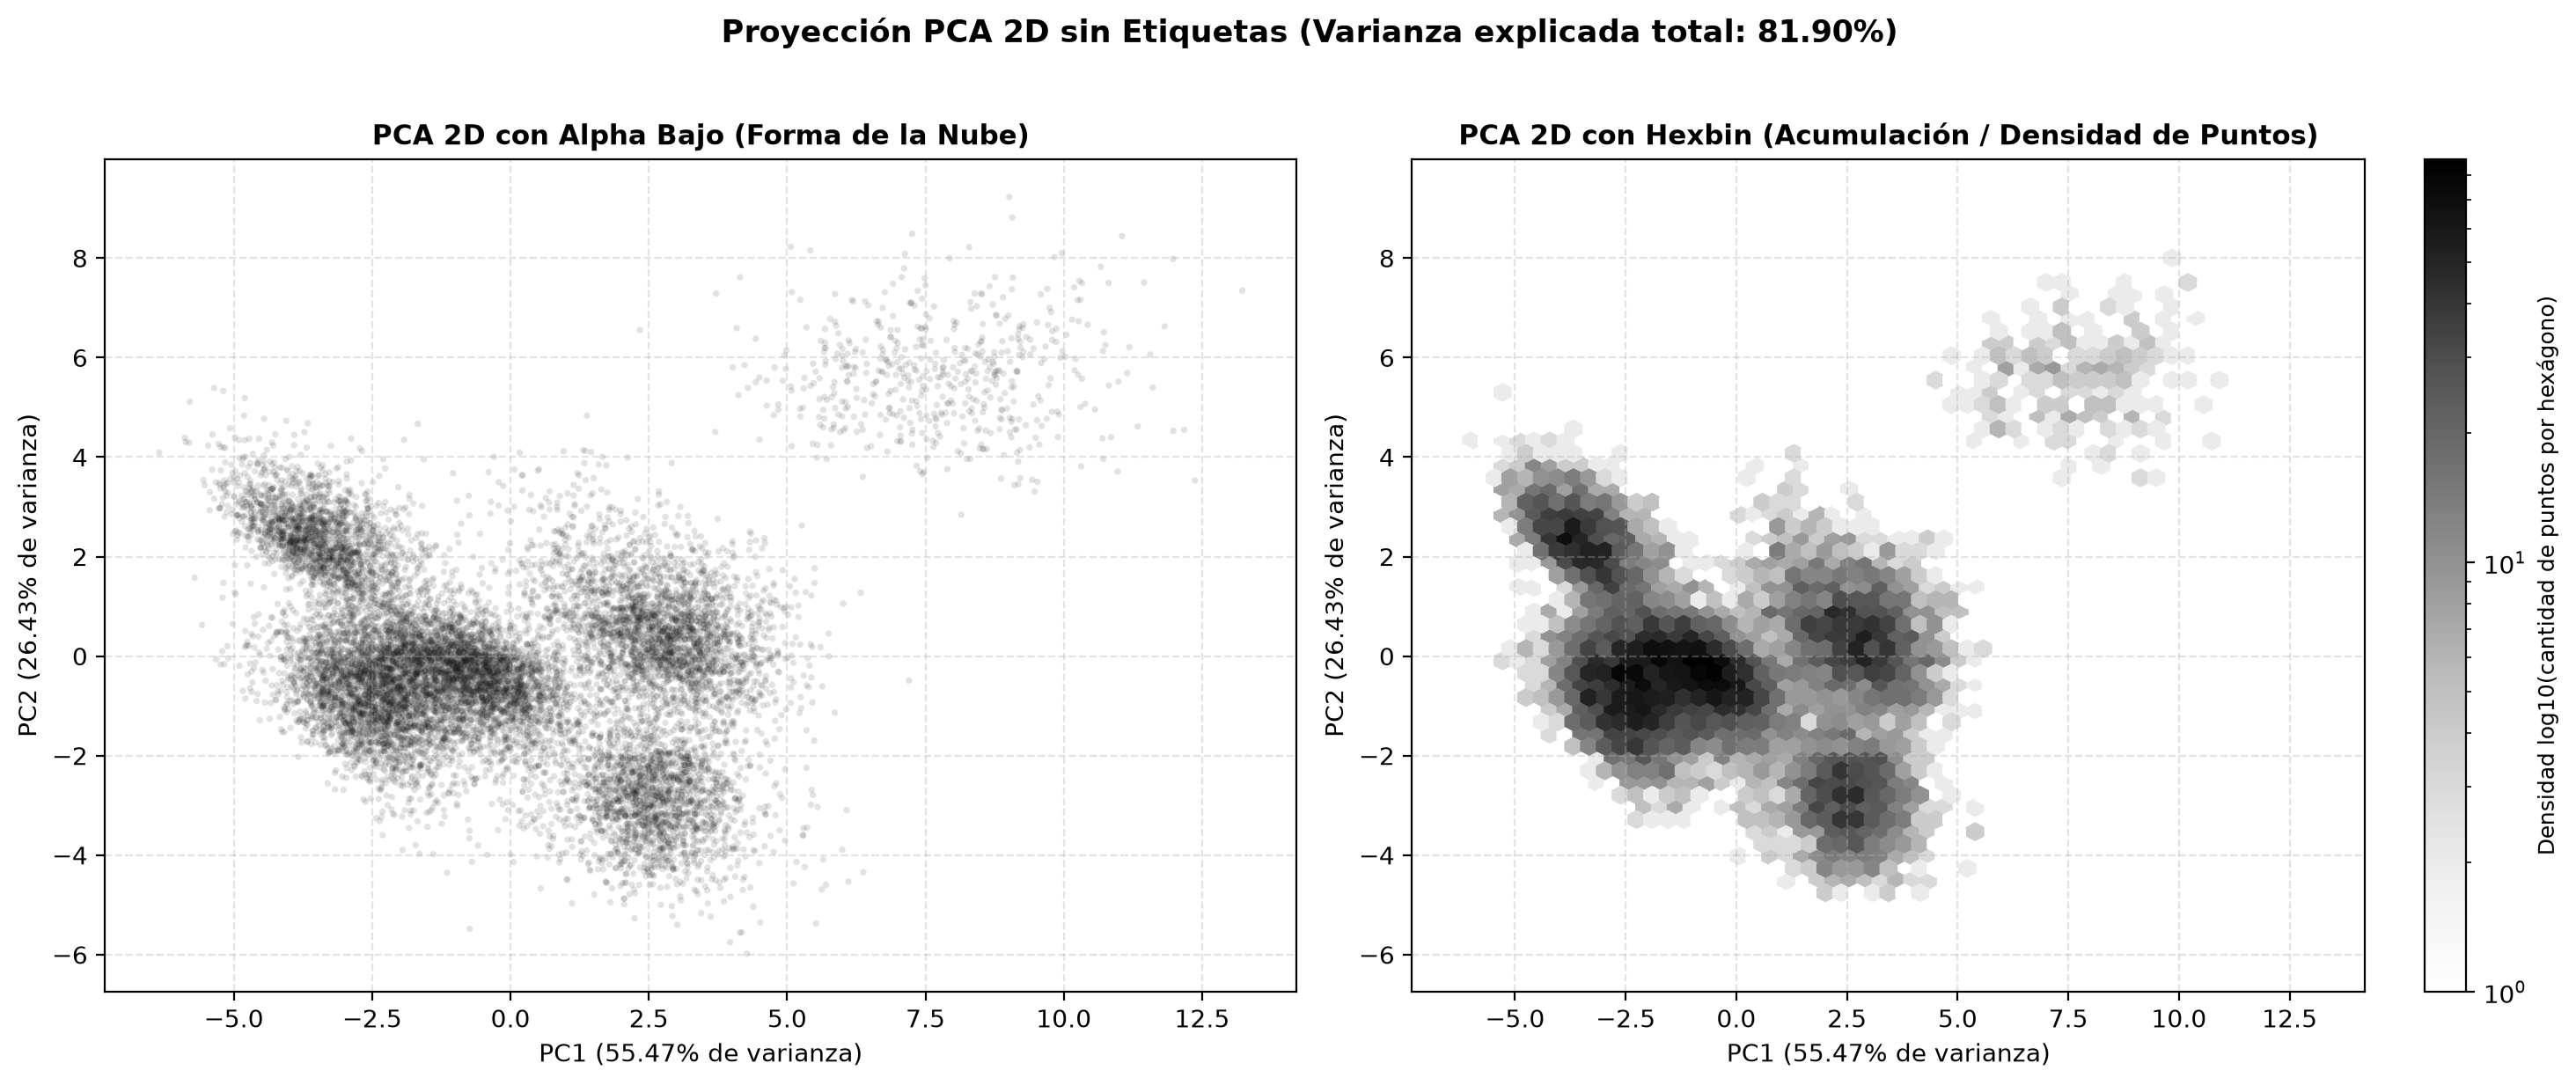
\includegraphics[width=0.98\textwidth]{Inciso_1/6_pca_2d_densidad.png}
    \caption{Proyección PCA 2D sin etiquetas (izquierda) y mapa de densidad Hexbin en escala logarítmica (derecha).}
    \label{fig:pca_analisis}
\end{figure}

\subsubsection*{2. Limpieza Inicial y Estandarización (\texttt{preprocesamiento.py})}

Con base en el diagnóstico anterior, el script \texttt{preprocesamiento.py} ejecuta la depuración inicial antes de aplicar DBSCAN:
\begin{enumerate}[leftmargin=0.8cm]
    \item \textbf{Eliminación de la columna vacía:} Se detecta dinámicamente y se elimina la columna \texttt{Unnamed: 16} (100\% nula), conservando las 16 variables numéricas válidas.
    \item \textbf{Eliminación de duplicados:} Se remueven las \textbf{68 filas repetidas}, quedando \textbf{13,543 registros únicos}.
    \item \textbf{Estandarización Z-score:} Se aplica \texttt{StandardScaler} ($z = \frac{x - \mu}{\sigma}$) sobre las 16 columnas para centrarlas en media $0.00$ y desviación estándar $1.00$ (Figura~\ref{fig:estandarizacion}), garantizando que todas las características contribuyan de manera equitativa al cálculo de distancias euclidianas.
\end{enumerate}

\begin{figure}[H]
    \centering
    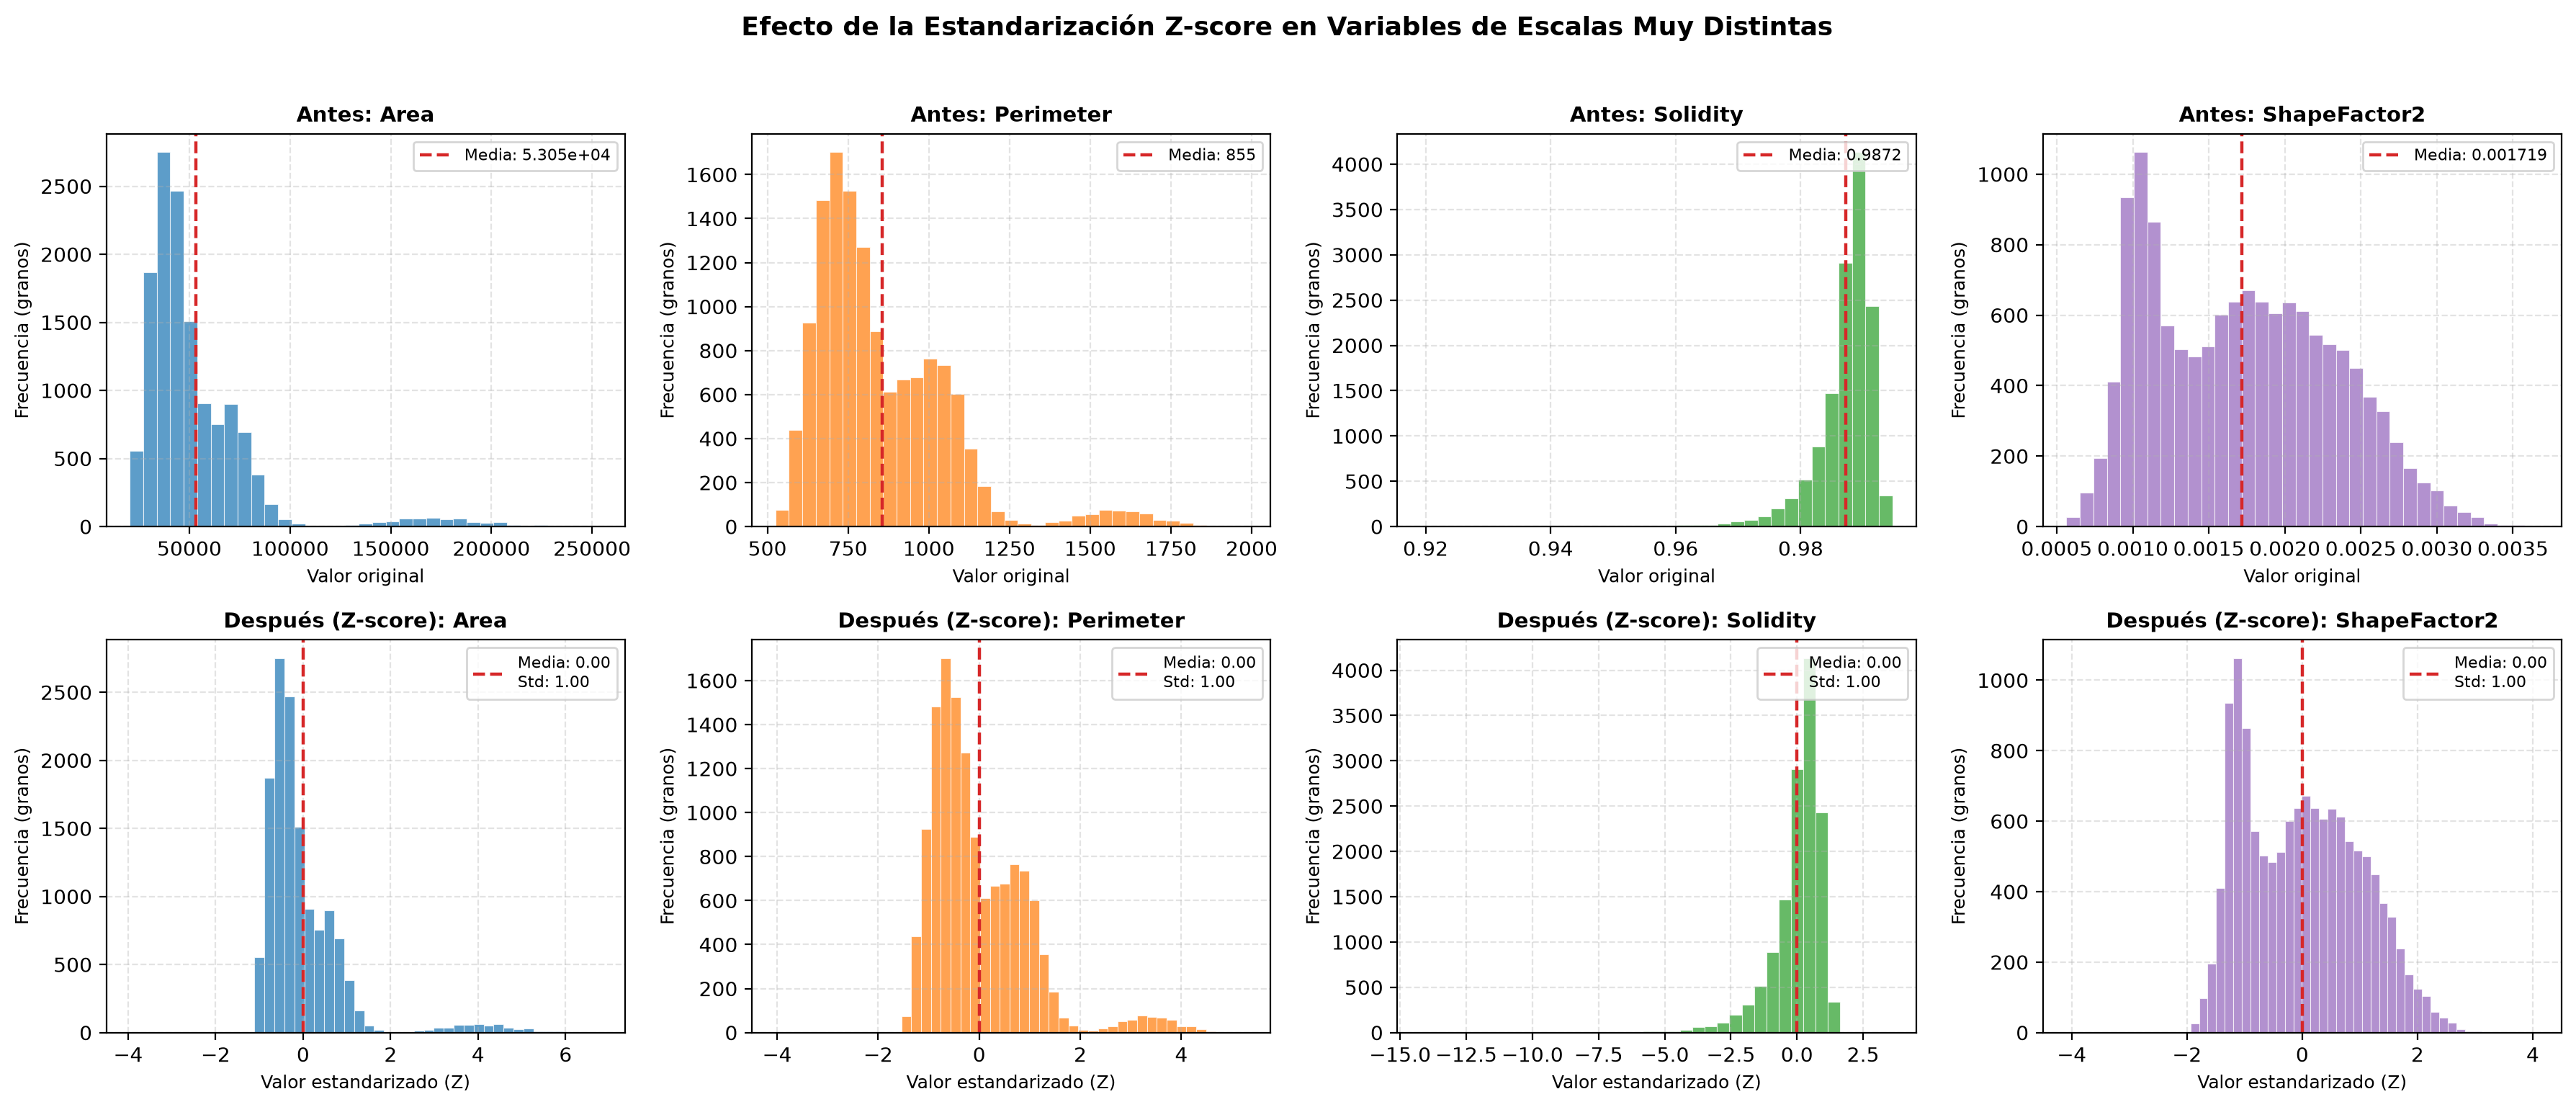
\includegraphics[width=0.98\textwidth]{Inciso_1/1_antes_despues_estandarizacion.png}
    \caption{Comparativa de escalas antes y después de aplicar la estandarización Z-score en variables representativas.}
    \label{fig:estandarizacion}
\end{figure}

\subsubsection*{3. Ajuste de DBSCAN y Elección de Métricas de Calidad}

Dado que las nubes de datos presentan formas irregulares, densidades variables y puntos aislados en las orillas, no se utilizaron filtros univariados por columna (como reglas $|Z| > 3$ o IQR, que recortarían granos grandes válidos) ni el algoritmo \textit{K-means} (que fuerza a todo punto a pertenecer a un grupo sin aislar el ruido). En su lugar, se utilizó \textbf{DBSCAN} directamente sobre las \textbf{16 dimensiones estandarizadas} con distancia euclidiana.

Para ajustar sus dos hiperparámetros principales se procedió de la siguiente manera:
\begin{itemize}[leftmargin=0.8cm]
    \item \textbf{Selección de $\text{MinPts} = 32$:} Siguiendo el criterio estándar para espacios multidimensionales de $D$ características, se fijó $\text{MinPts} = 2 \times D = 2 \times 16 = 32$ vecinos mínimos para definir una región densa.
    \item \textbf{Curva de $k$-distancias para $\varepsilon$:} Se calculó la distancia euclidiana al vecino número 32 más cercano para cada grano y se ordenaron las distancias de menor a mayor (Figura~\ref{fig:k_dist}). El cambio abrupto de pendiente (zona del codo) se ubicó entre los percentiles 90 y 95 (\texttt{P90} $= 1.42$ y \texttt{P95} $= 1.76$), delimitando el intervalo donde comienzan los puntos dispersos candidatos a ruido global.
\end{itemize}

\begin{figure}[H]
    \centering
    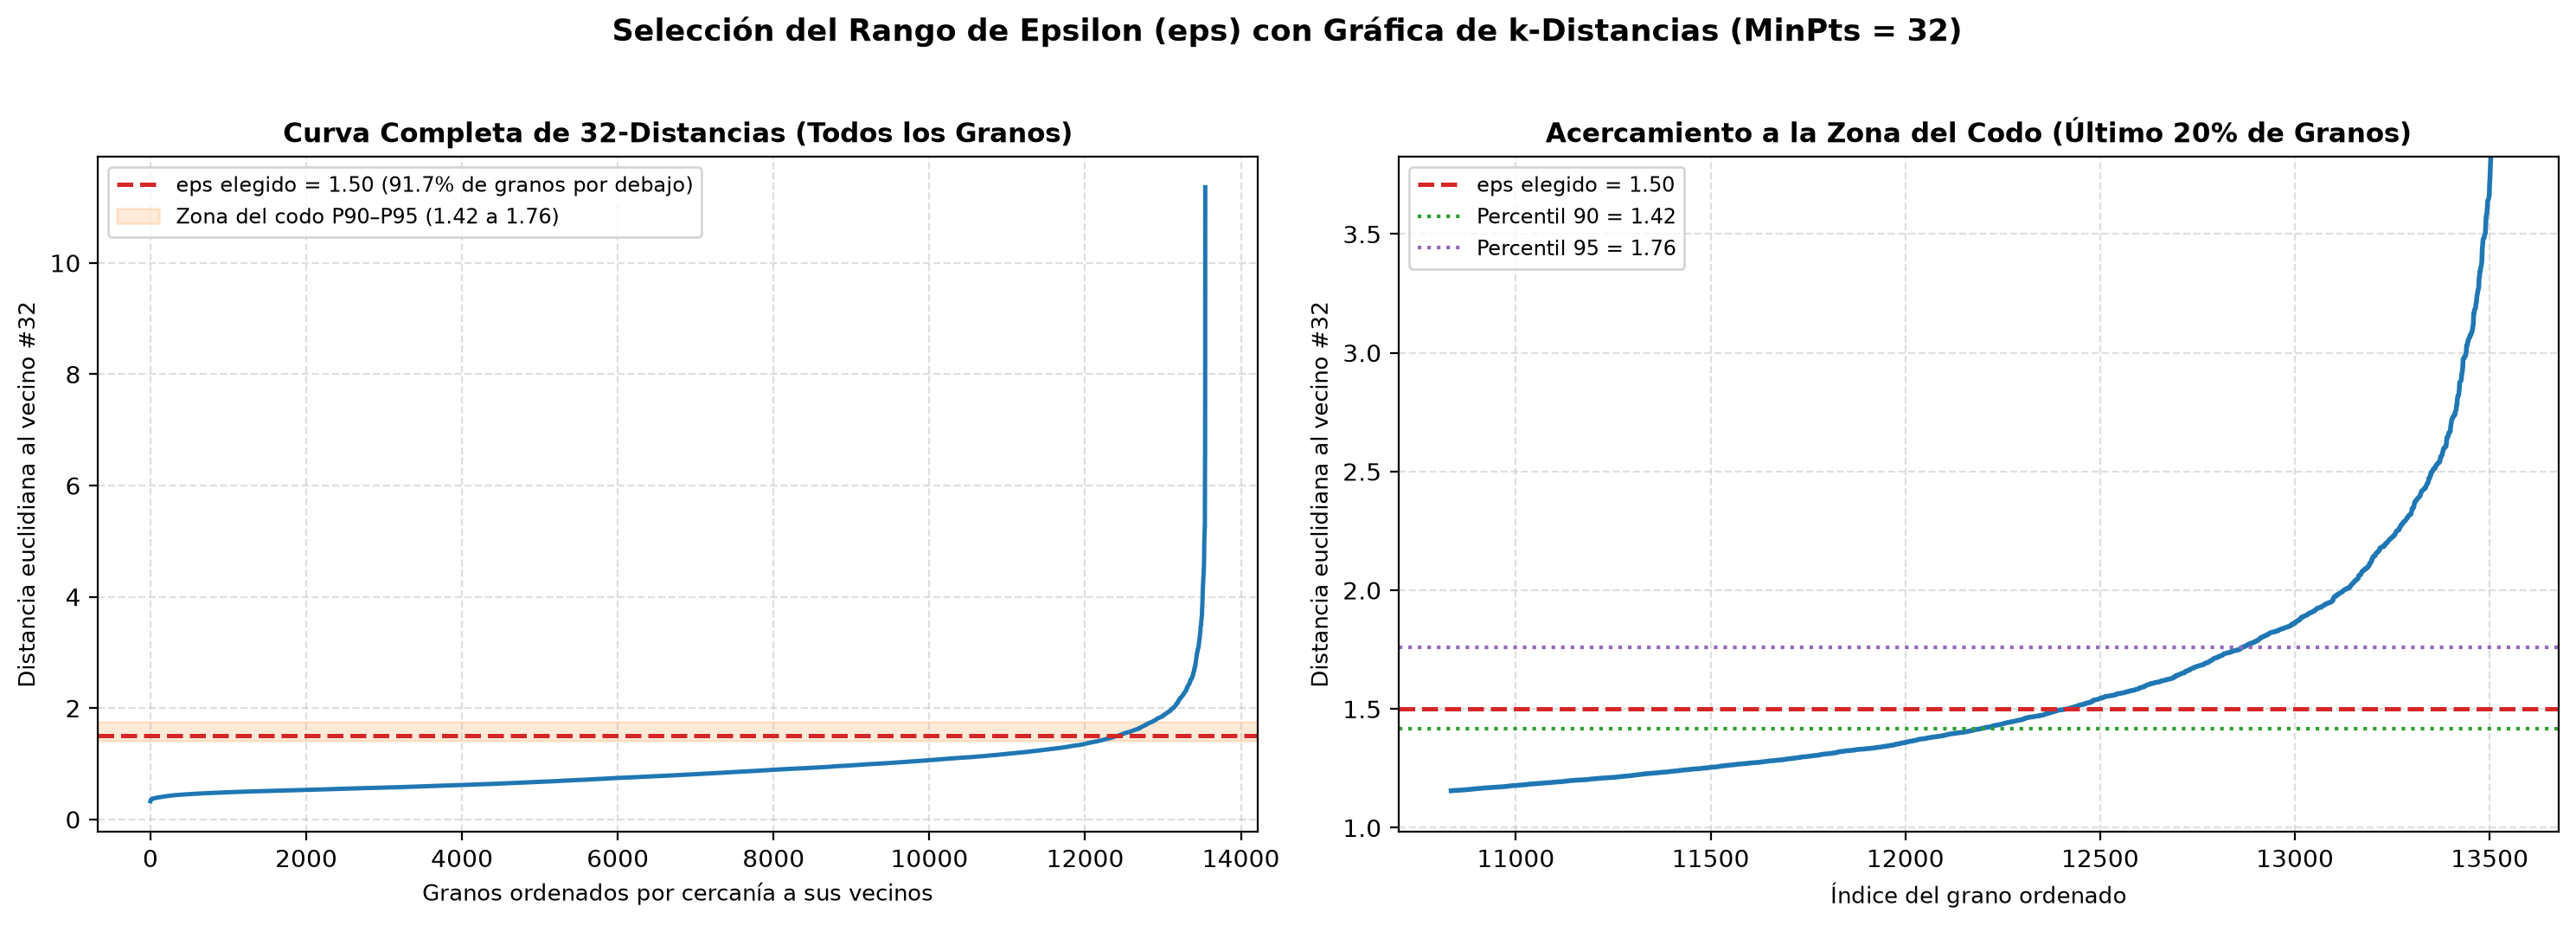
\includegraphics[width=0.98\textwidth]{Inciso_1/2_curva_k_distancia_dbscan.png}
    \caption{Curva de 32-distancias ordenadas para identificar el intervalo del codo de $\varepsilon$.}
    \label{fig:k_dist}
\end{figure}

Posteriormente se evaluaron distintos valores de $\varepsilon$ alrededor de la zona del codo utilizando \textbf{métricas de validación interna para agrupamiento no supervisado} (excluyendo métricas externas como ARI o NMI porque no existen etiquetas previas, así como la inercia por ser propia de \textit{K-means}):
\begin{itemize}[leftmargin=0.8cm]
    \item \textbf{Silhouette Score} (cercano a $1$ es mejor): evalúa cohesión interna y separación entre clusters.
    \item \textbf{Davies-Bouldin Index} (menor es mejor): mide la relación entre dispersión intra-cluster y distancia entre centroides.
    \item \textbf{Calinski-Harabasz Index} (mayor es mejor): mide la razón entre dispersión inter-cluster e intra-cluster.
    \item \textbf{Número de clusters y porcentaje de ruido global ($-1$):} controla el equilibrio entre limpieza de puntos aislados y preservación de datos válidos.
\end{itemize}

\begin{table}[H]
    \centering
    \caption{Resultados de la evaluación de métricas internas en DBSCAN con $\text{MinPts} = 32$.}
    \label{tab:metricas_dbscan}
    \begin{tabular}{@{} c c c r r c c c @{}}
        \toprule
        $\varepsilon$ (\texttt{eps}) & \texttt{MinPts} & Clusters & Ruido ($-1$) & \% Ruido & Silhouette ($\uparrow$) & Davies-Bouldin ($\downarrow$) & Calinski-Harabasz ($\uparrow$) \\
        \midrule
        $0.90$ & $32$ & $3$ & $2{,}941$ & $21.72\%$ & $0.2416$ & $0.9698$ & $2{,}108.1$ \\
        $1.20$ & $32$ & $2$ & $934$   & $6.90\%$  & $0.5731$ & $0.4766$ & $2{,}515.2$ \\
        $1.40$ & $32$ & $2$ & $515$   & $3.80\%$  & $0.5692$ & $0.5072$ & $3{,}404.8$ \\
        \textbf{1.50} & \textbf{32} & \textbf{2} & \textbf{402} & \textbf{2.97\%} & \textbf{0.5703} & \textbf{0.5136} & \textbf{3,664.6} \\
        $1.60$ & $32$ & $2$ & $322$   & $2.38\%$  & $0.5700$ & $0.5192$ & $3{,}822.4$ \\
        $1.80$ & $32$ & $2$ & $204$   & $1.51\%$  & $0.5697$ & $0.5283$ & $4{,}001.6$ \\
        $2.00$ & $32$ & $2$ & $128$   & $0.95\%$  & $0.5707$ & $0.5356$ & $4{,}169.6$ \\
        \bottomrule
    \end{tabular}
\end{table}

\begin{figure}[H]
    \centering
    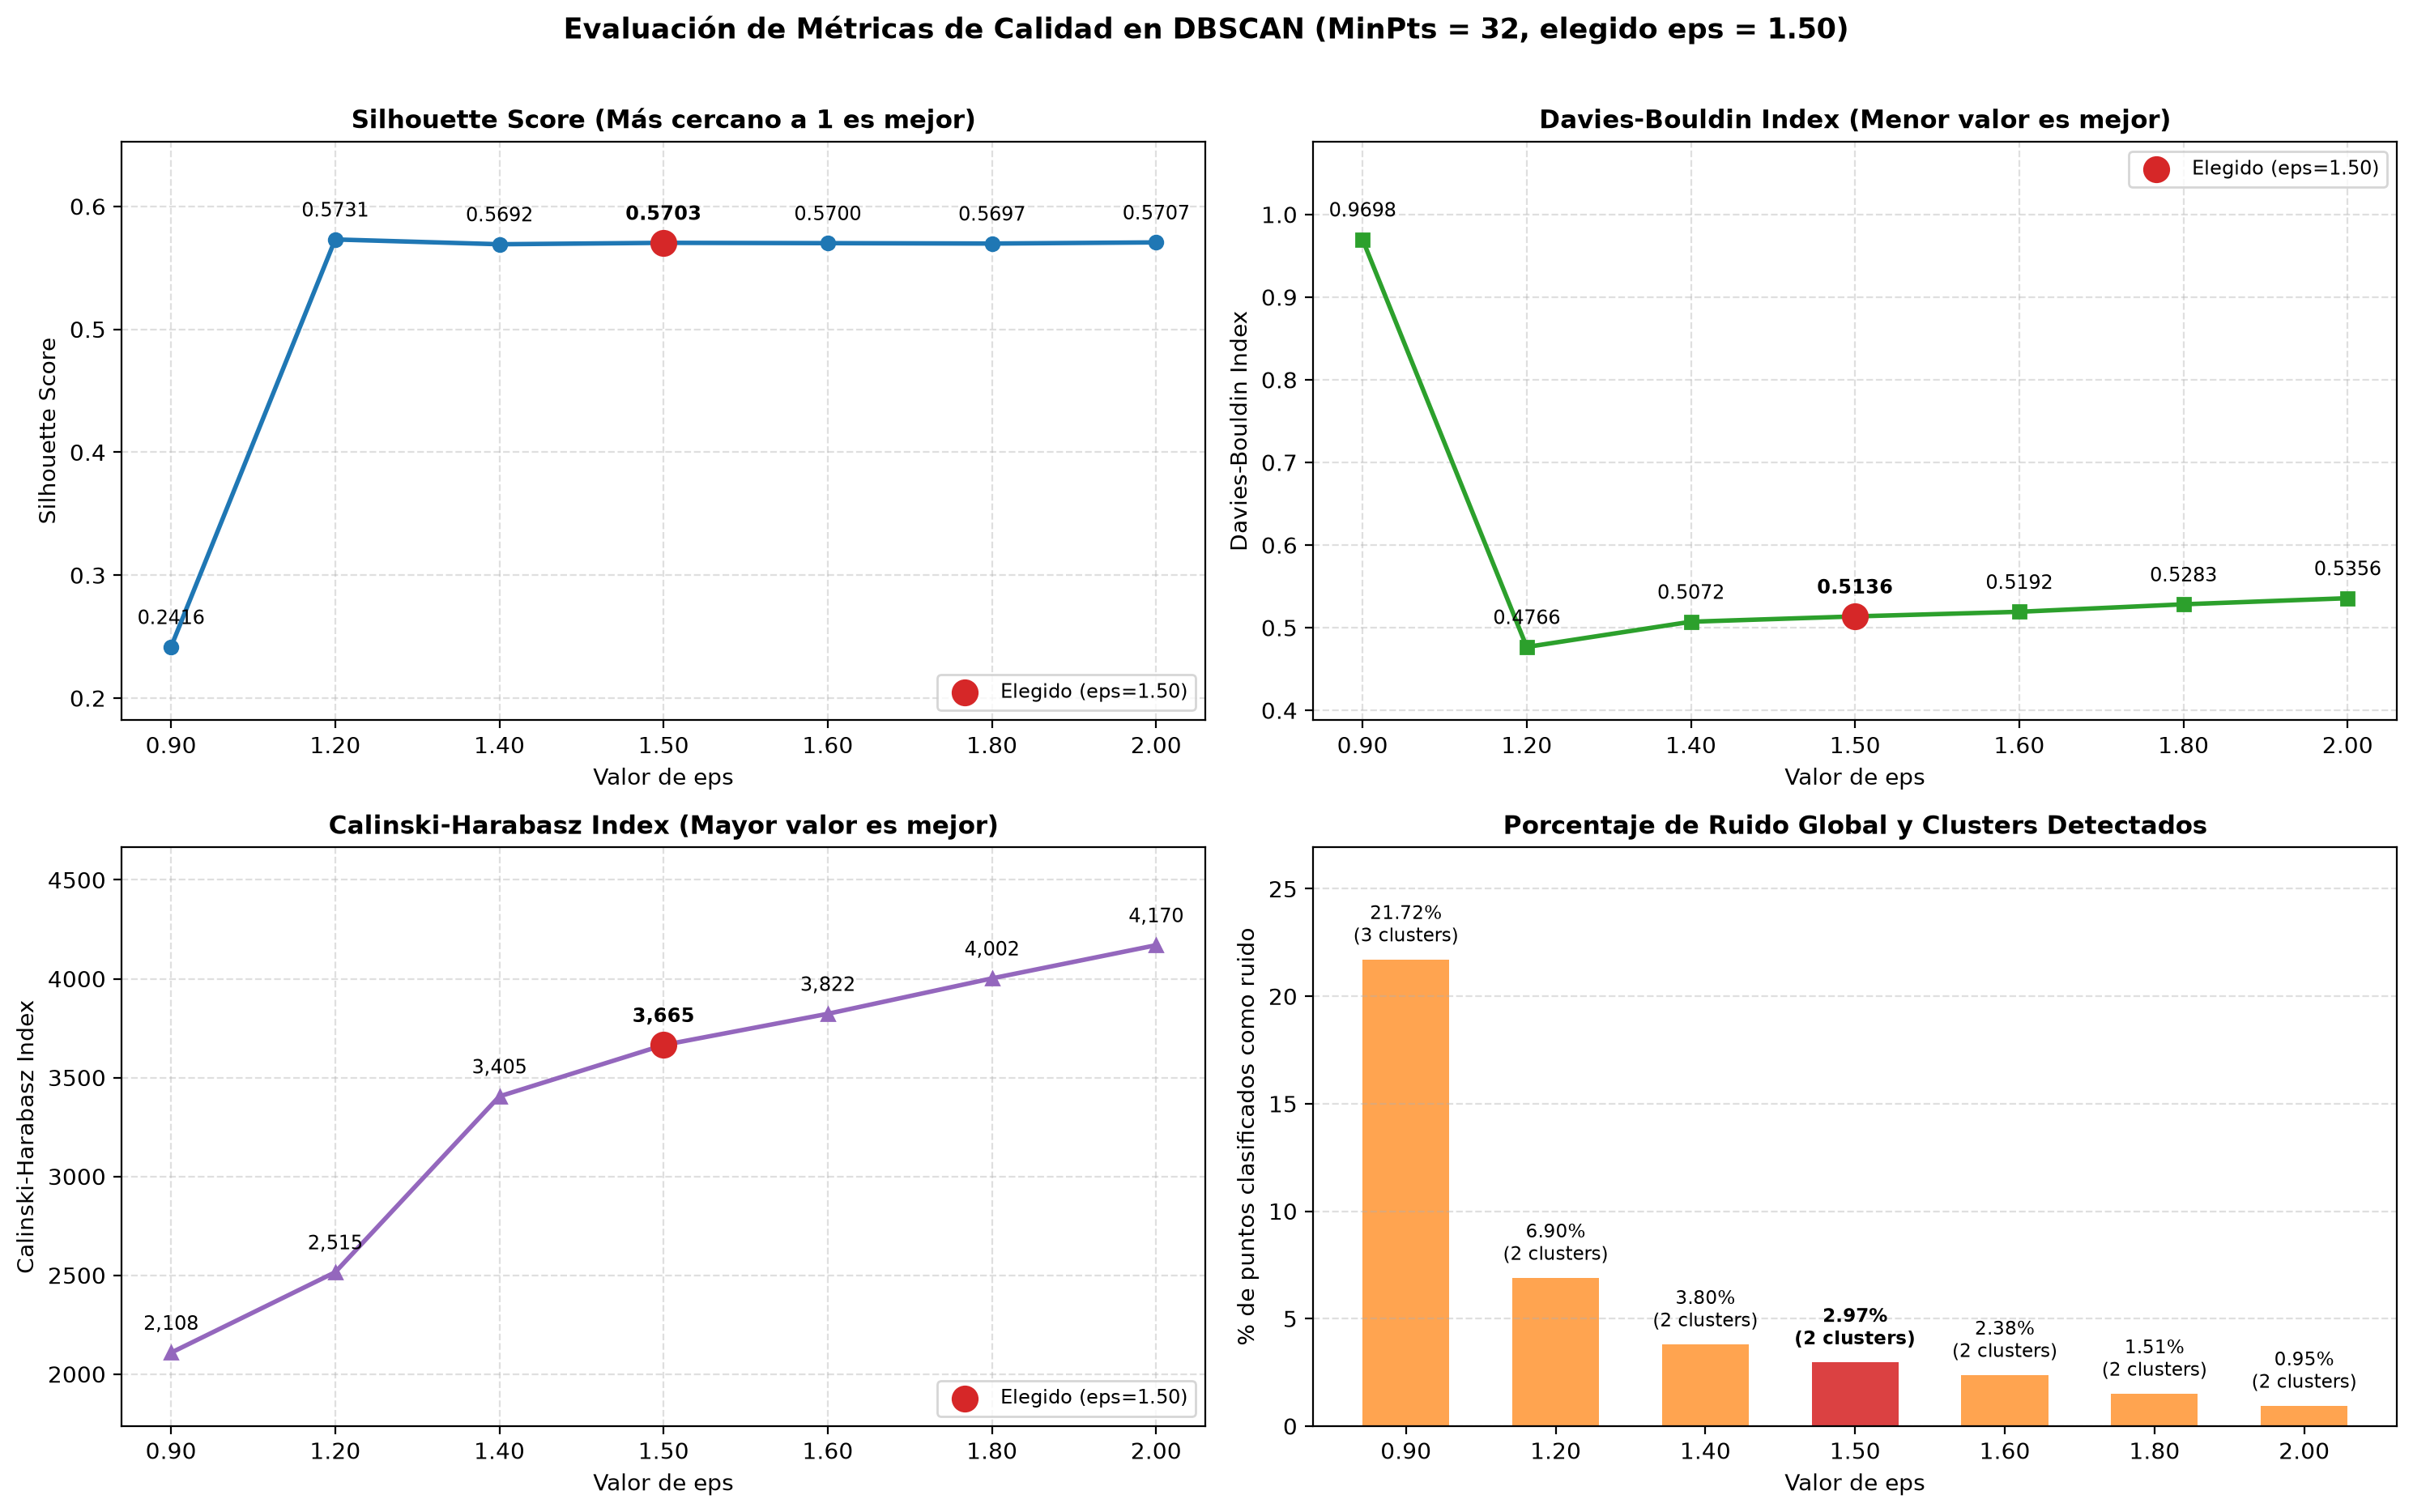
\includegraphics[width=0.98\textwidth]{Inciso_1/3_metricas_calidad_dbscan.png}
    \caption{Comportamiento comparativo de las métricas de calidad de DBSCAN al variar el parámetro $\varepsilon$.}
    \label{fig:metricas_dbscan}
\end{figure}

Como se observa en la Tabla~\ref{tab:metricas_dbscan} y en la Figura~\ref{fig:metricas_dbscan}, con radios pequeños ($\varepsilon = 0.90$) se pierde más del 21\% del dataset y la calidad cae drásticamente (\texttt{Silhouette} $= 0.2416$); mientras que con radios grandes ($\varepsilon = 2.00$) el índice Davies-Bouldin se deteriora ($0.5356$) al absorber puntos periféricos. El script selecciona automáticamente dentro del codo [\texttt{P90}, \texttt{P95}] la configuración \textbf{$\varepsilon = 1.50$, $\text{MinPts} = 32$}, que logra el mejor equilibrio con \textbf{2 clusters bien separados} (\texttt{Silhouette} $= 0.5703$, \texttt{Davies-Bouldin} $= 0.5136$, \texttt{Calinski-Harabasz} $= 3{,}664.6$) y elimina únicamente \textbf{402 registros de ruido global (2.97\%)}.

\subsubsection*{4. Eliminación del Ruido Global y Asignación de Clases}

En la Figura~\ref{fig:comparativa_dbscan} se muestra el efecto de aplicar DBSCAN sobre las 16 variables (proyectado en PCA 2D únicamente para su visualización): las 4 zonas densas de la nube principal quedan conectadas como un solo estrato continuo (\textbf{Cluster 0}, en azul) debido a que comparten puentes de densidad en 16D (forzar su separación con $\varepsilon \approx 0.70$--$0.80$ eliminaría entre el 32\% y 45\% del conjunto de datos como ruido), mientras que la nube de granos grandes forma un grupo independiente (\textbf{Cluster 1}, en naranja) y los 402 puntos dispersos de las orillas quedan marcados en rojo ($-1$) y son eliminados.

\begin{figure}[H]
    \centering
    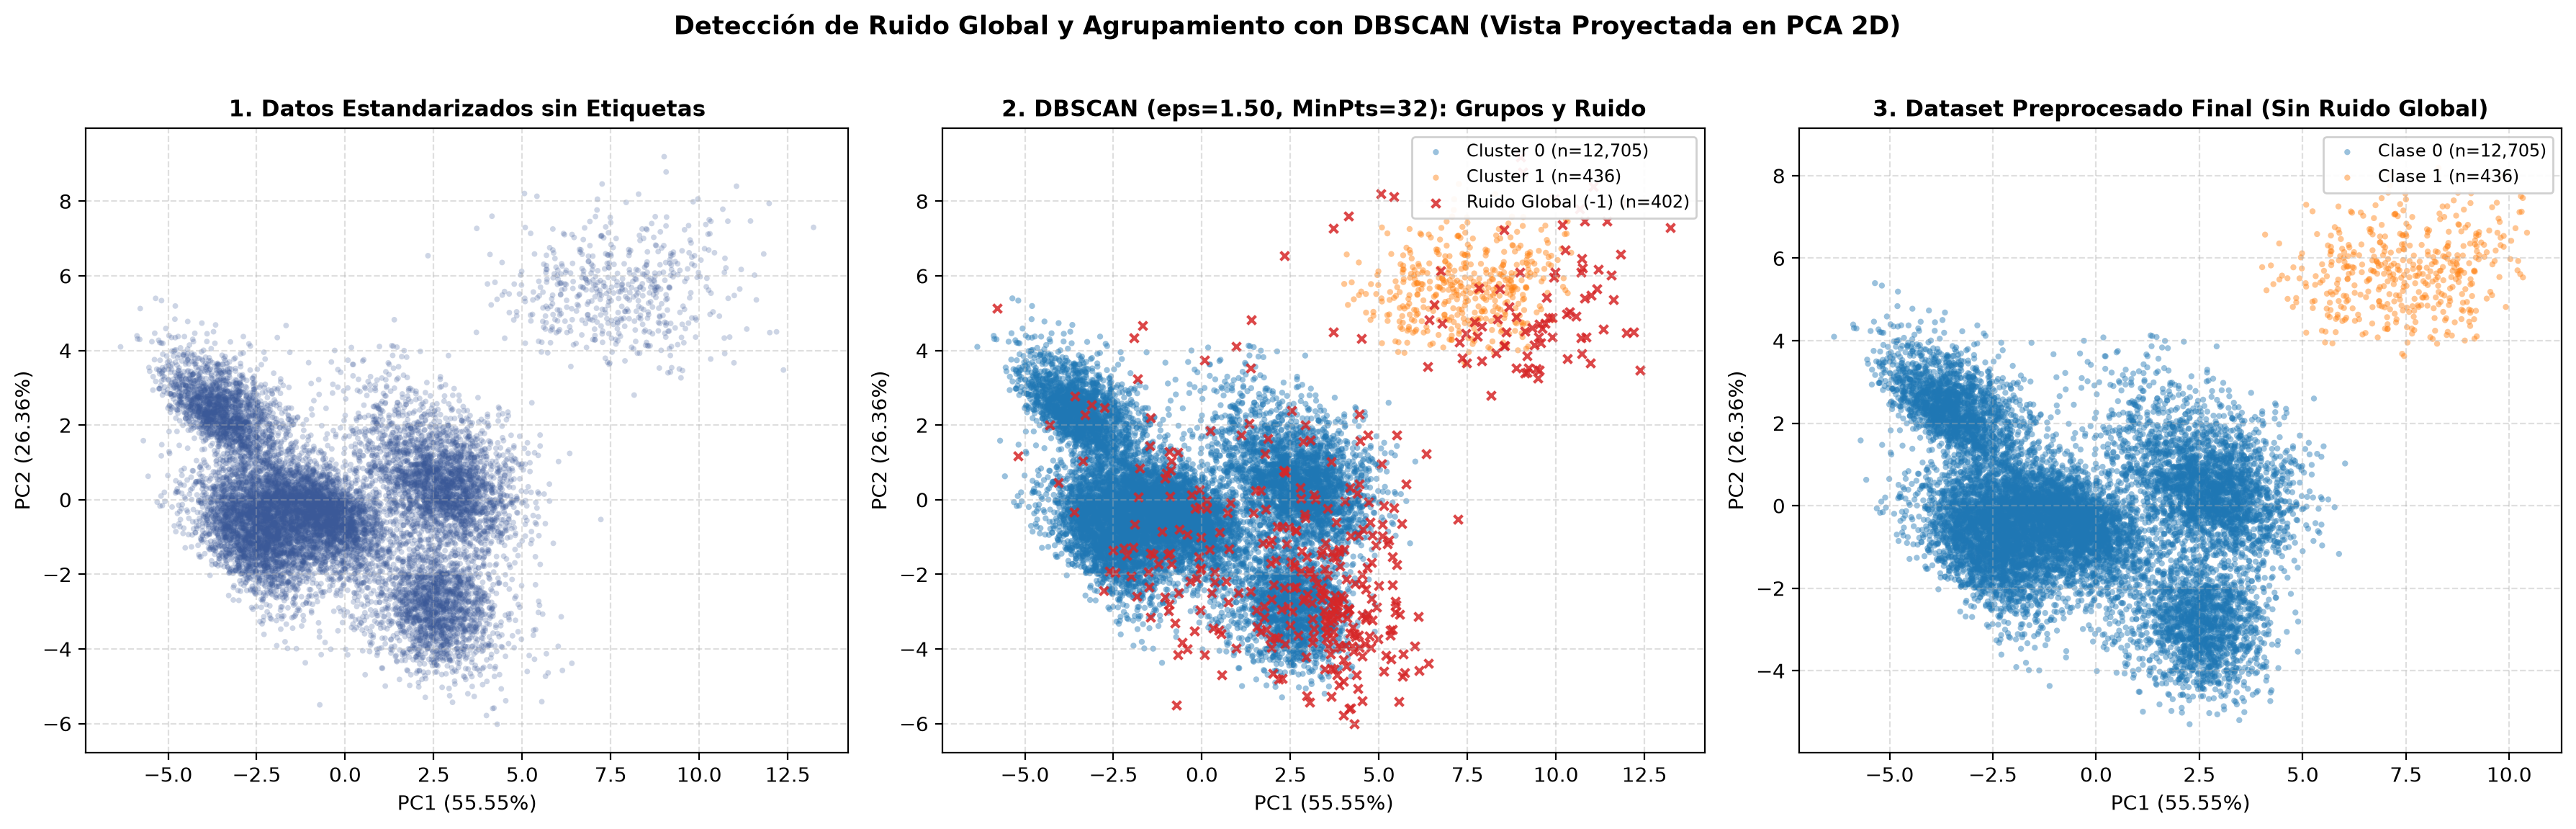
\includegraphics[width=0.98\textwidth]{Inciso_1/4_dbscan_clustering_y_ruido.png}
    \caption{Comparativa antes, durante (identificación de ruido global en cruces rojas) y después de limpiar el dataset con DBSCAN.}
    \label{fig:comparativa_dbscan}
\end{figure}

Finalmente, a los registros limpios se les asignó el identificador del cluster descubierto en la columna \textbf{\texttt{Clase}} y se exportó el resultado al archivo \texttt{dataset\_preprocesado.csv} con dimensiones de \textbf{13,141 filas $\times$ 17 columnas} (16 atributos estandarizados más la columna \texttt{Clase}), distribuidos como se muestra en la Figura~\ref{fig:resumen_final}:
\begin{itemize}[leftmargin=0.8cm]
    \item \textbf{\texttt{Clase 0}:} 12,705 granos (\textbf{96.68\%}).
    \item \textbf{\texttt{Clase 1}:} 436 granos (\textbf{3.32\%}).
\end{itemize}

\begin{figure}[H]
    \centering
    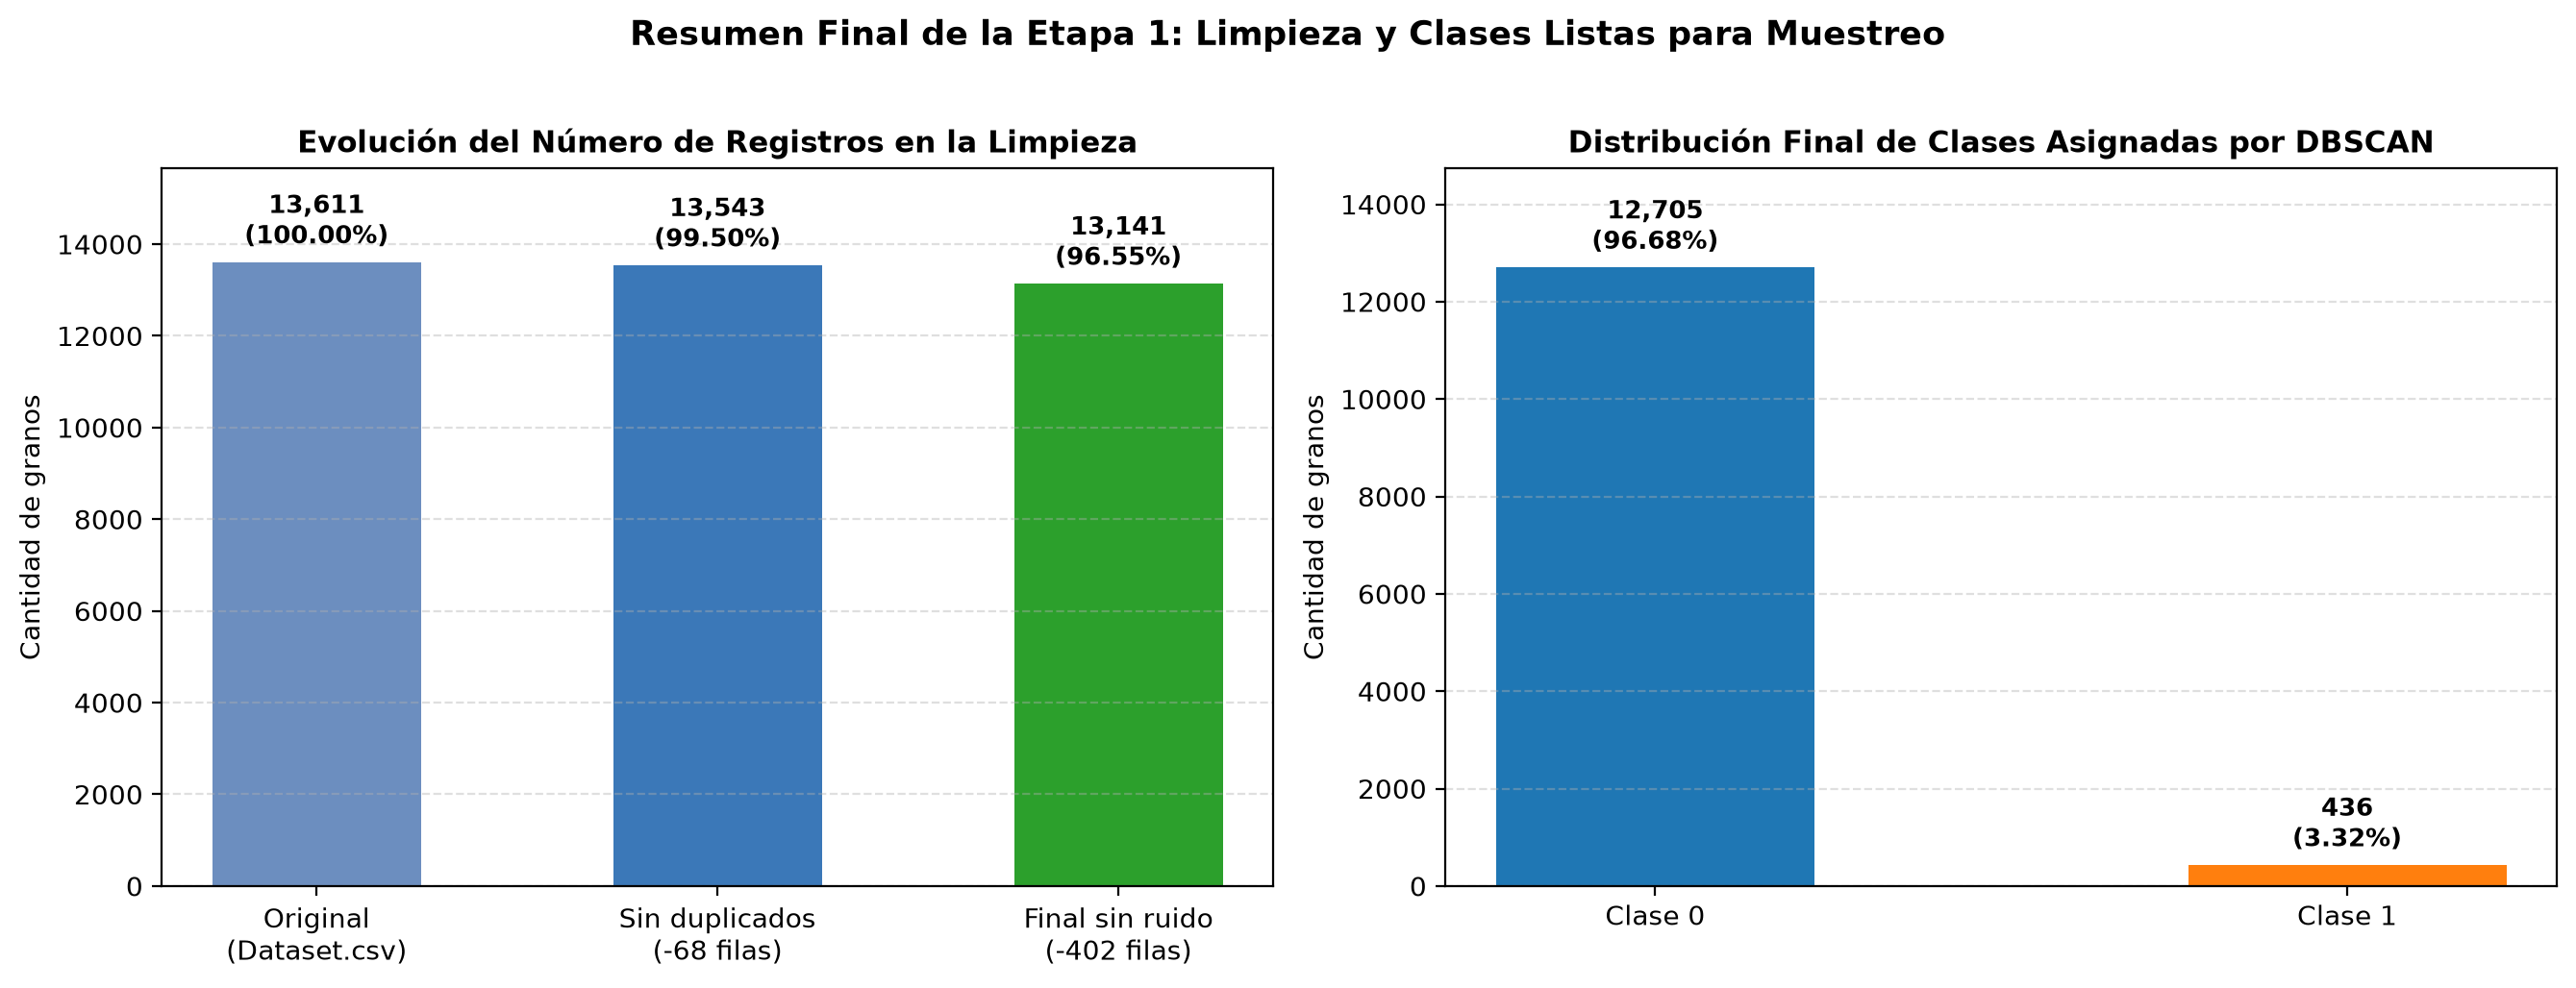
\includegraphics[width=0.95\textwidth]{Inciso_1/5_resumen_preprocesamiento_y_clases.png}
    \caption{Reducción progresiva de registros durante la limpieza y distribución final de las clases asignadas.}
    \label{fig:resumen_final}
\end{figure}

Este archivo limpio y etiquetado constituye la entrada directa para la etapa de muestreo estratificado (Etapa 2), indispensable para preservar la proporción de la clase minoritaria ($3.32\%$) en los conjuntos de entrenamiento, validación y prueba de la Red Neuronal.

\end{document}
